% T-CNS flagship §VIII (numerics) — Tier-1-ONLY rendition per the publication
% split (R9 defense: the multibody campaign is the RA-L companion; a forward
% pointer only appears here). \input into the flagship, or compile
% standalone.tex to preview. Registry captions verbatim where mandated.
\section{Numerical verification}\label{sec:numerics}

All cells in this section run on the reduced plant inside protocol class
$\mathcal{P}$ (uniform lags, zero jitter and loss, realized age asserted equal
to $\tau$ per fusion event), with the estimator, metric functional, window
rules, and fit code shared verbatim with the multibody companion --- so
agreement between the two papers is a statement about the algorithm, and
disagreement localizes to the plant. Every claim below carries the pre-registered
falsifier it was exposed to; three fired, and their firings are reported as
findings. Every number traces to a seeded, versioned driver re-executed
exactly by the released replay harness.

\subsection{Gauge structure and pinning (E1; Thm.~\ref{thm:gaugeF}, Cor.~\ref{cor:pinF})}
On the triangle with generic shapes, the sheaf Laplacian is PSD with
$\dim\ker L_\mathcal{F} = 3$ and the gauge section
$(\mathrm{Ad}^{-1}_{m(s_j)} c)_j$ annihilated to $1.3\times10^{-15}$;
$\sigma_4/\sigma_3$ confirms a clean spectral gap. Adding a single anchor
potential collapses the kernel to zero and $\lambda_{\min}$ becomes the
convergence rate --- the pinning corollary as linear algebra
(Fig.~\ref{fig:f3}).
\begin{figure}[t]
  \centering
  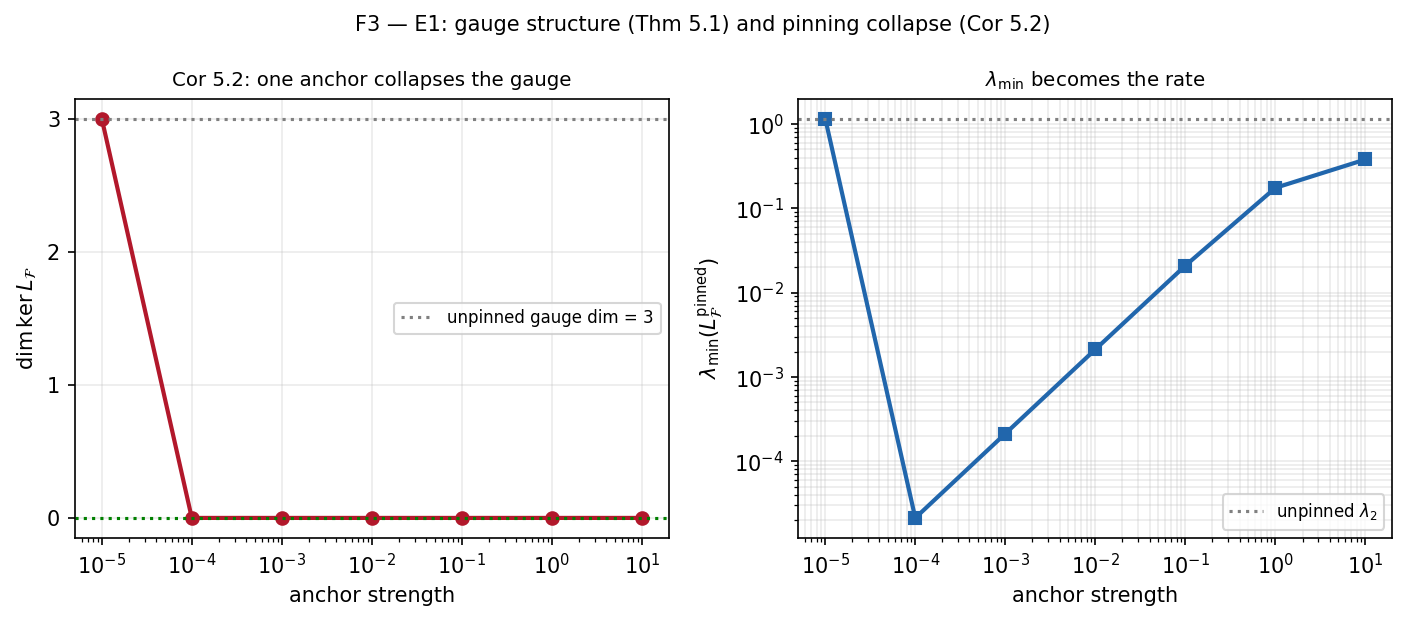
\includegraphics[width=\linewidth]{figures/e1_gauge.png}
  \caption{Gauge spectrum: $\dim\ker L_\mathcal{F} = 3$ with the harmonic
  sections exactly the body-framed images of one common load-frame
  perturbation; one anchor removes the kernel.}
  \label{fig:f3}
\end{figure}

\subsection{The theorem's object: amplitude, coefficient, switch-offs
(E3a; Thm.~\ref{thm:floorF})}
The measured amplitude $\|\mathrm{Log\,Hol}\|$ on the $m{=}2$ round trip fits
slope $1.999$ over $\tau \in [0.05, 1.6]$\,s with coefficient ratio
$\|\mathrm{Log\,Hol}\|/\tau^2\|[C_i,C_j]\| = 1.0000$ at the smallest $\tau$;
the switch-off arms sit at machine zero ($s_i{\equiv}s_j$: $<10^{-15}$;
$\eta{=}0$: $<10^{-17}$; $\xi{=}0$: exactly $0.0$; explicit $\tau{=}0$ arm:
exactly $0.0$). Four extension arms sharpen this (Fig.~\ref{fig:f4aext}):
the slope is formation-invariant across 20 random taut formations
($1.9993 \pm 0.0000$); the remainder constant is uniformly tight
($\sup_{s,\tau} \|R\|/\tau^3 \le 0.0133$ over 220 draws); and a search for
zero-commutator pairs at $\ge 1$\,rad shape separation found only pairs with
$C_i = C_j$ to $10^{-16}$ --- the protected class of
Cor.~\ref{cor:symF} extends, empirically, to the level set of
$s \mapsto C(s;\xi)$, where the full holonomy vanishes at all orders.
\begin{figure}[t]
  \centering
  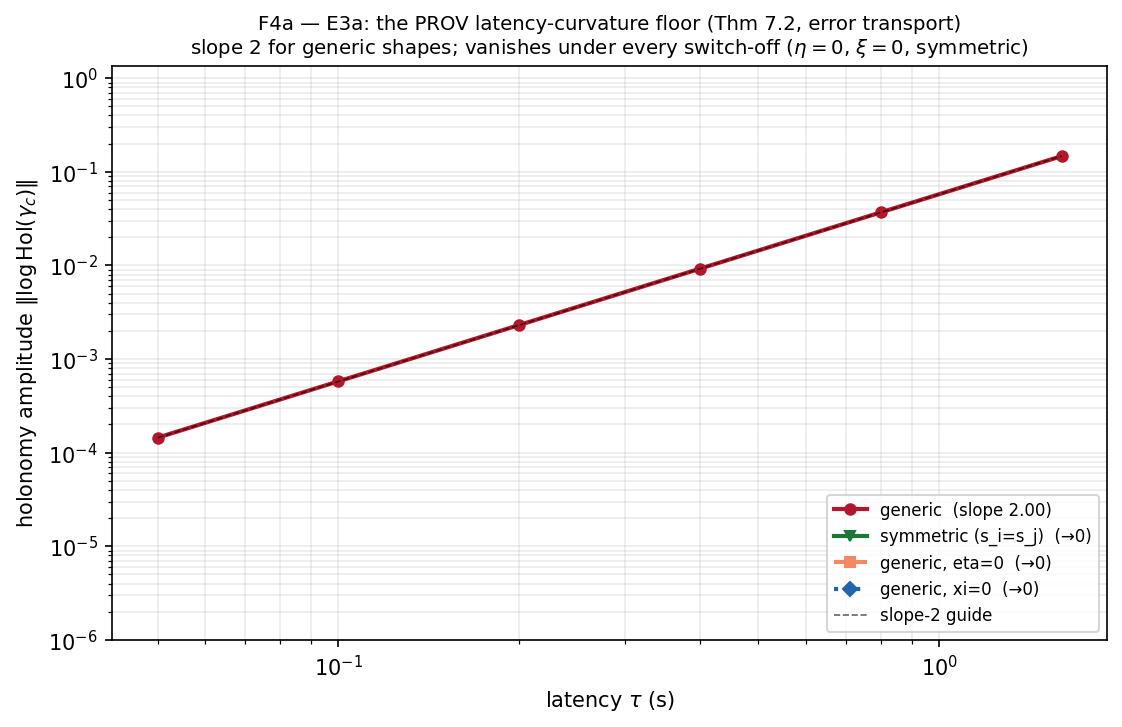
\includegraphics[width=\linewidth]{figures/e3a_amplitude.png}
  \caption{F4a: the leading-order, deterministic holonomy amplitude of
  Thm.~\ref{thm:floorF} --- slope 1.999, coefficient 1.0000, switch-offs at
  machine zero.}
  \label{fig:f4a}
\end{figure}
\begin{figure}[t]
  \centering
  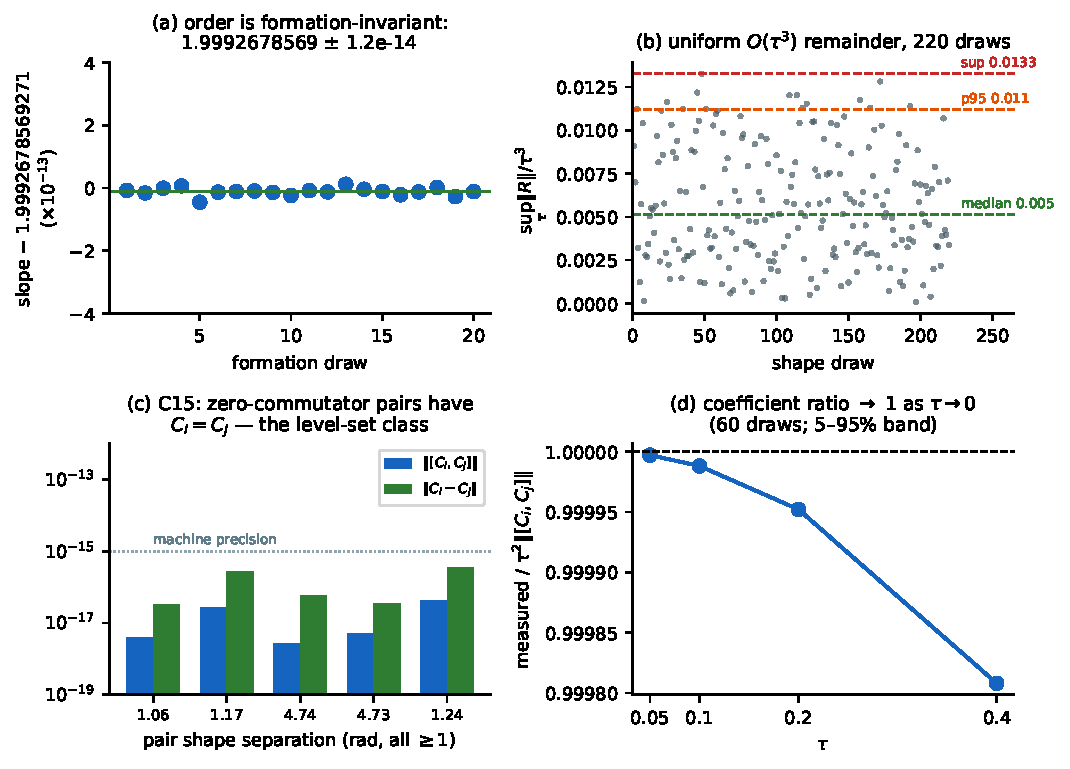
\includegraphics[width=\linewidth]{figures/e3a_extension_panels.pdf}
  \caption{E3a extension arms: formation-invariant order; uniform
  $O(\tau^3)$ remainder; the level-set symmetry class; coefficient ratio
  $\to 1$.}
  \label{fig:f4aext}
\end{figure}

\subsection{The conjectured closed-loop floor, falsified in its own regime
(E3b)}
\begin{figure}[t]
  \centering
  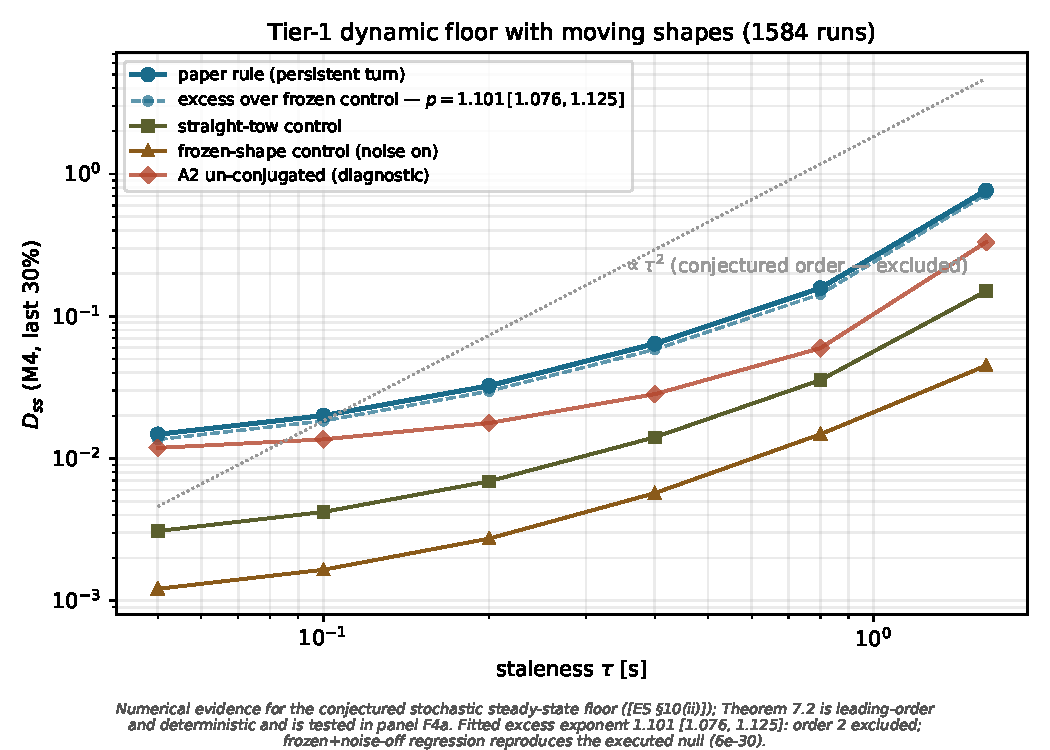
\includegraphics[width=\linewidth]{figures/f4b_tier1.pdf}
  \caption{Numerical evidence for the conjectured stochastic steady-state
  floor ([ES \S10(ii)]); Theorem~\ref{thm:floorF} is leading-order and
  deterministic and is tested in Fig.~\ref{fig:f4a}. Fitted excess exponent
  1.101 [1.076, 1.125]: the conjectured order 2 is excluded (and so is 1);
  the frozen+noise-off regression reproduces the executed null
  ($D_{ss} \sim 10^{-30}$).}
  \label{fig:f4b}
\end{figure}
With the full DIEKF-$\Sigma$ on the reduced plant integrating the shape ODEs
along the persistent-turn reference (1584 runs; 12 formations $\times$ 10
seeds per $\tau$ point; controls on matched draws), the disagreement excess
over the frozen-shape control fits exponent $1.101\,[1.076, 1.125]$
(formation-cluster CI $[1.070, 1.132]$): the \conjtag{} extension of the floor
to the noisy closed loop is falsified at these scales, coherently with the
multibody companion (cross-tier exponent difference $+0.023\,[-0.012,
+0.057]$). The mechanism check passes --- straight-tow and frozen controls
sit $5$--$13\times$ and further below --- and the executed null pins the
harness: shapes frozen and noise off give $D_{ss} \sim 10^{-30}$.

\subsection{Symmetry: two metrics, two exponents (E3c; Cor.~\ref{cor:symF})}
The amplitude departure from the symmetric class is first-order in
$\varepsilon$ (measured 1.006; base commutator exactly zero). The closed-loop
floor excess under the seed-paired estimator fits $\varepsilon$-exponent
$1.58\,[1.44, 1.84]$ at every $\tau$ --- excluding both the conjectured 2 and
1, with segment slopes rising $1.2 \to 2.1$ up the ladder: a
linear-plus-quadratic mixture that the registered single-power model
mis-specifies (reported per the outcome ladder). The robust
$\ge 10\times$ suppression falsifier trips ($2.75\times\,[1.94, 3.89]$ under
20\% jitter and 10\% loss): large symmetric protection is a property of the
amplitude object only (Fig.~\ref{fig:f5tc}).
\begin{figure}[t]
  \centering
  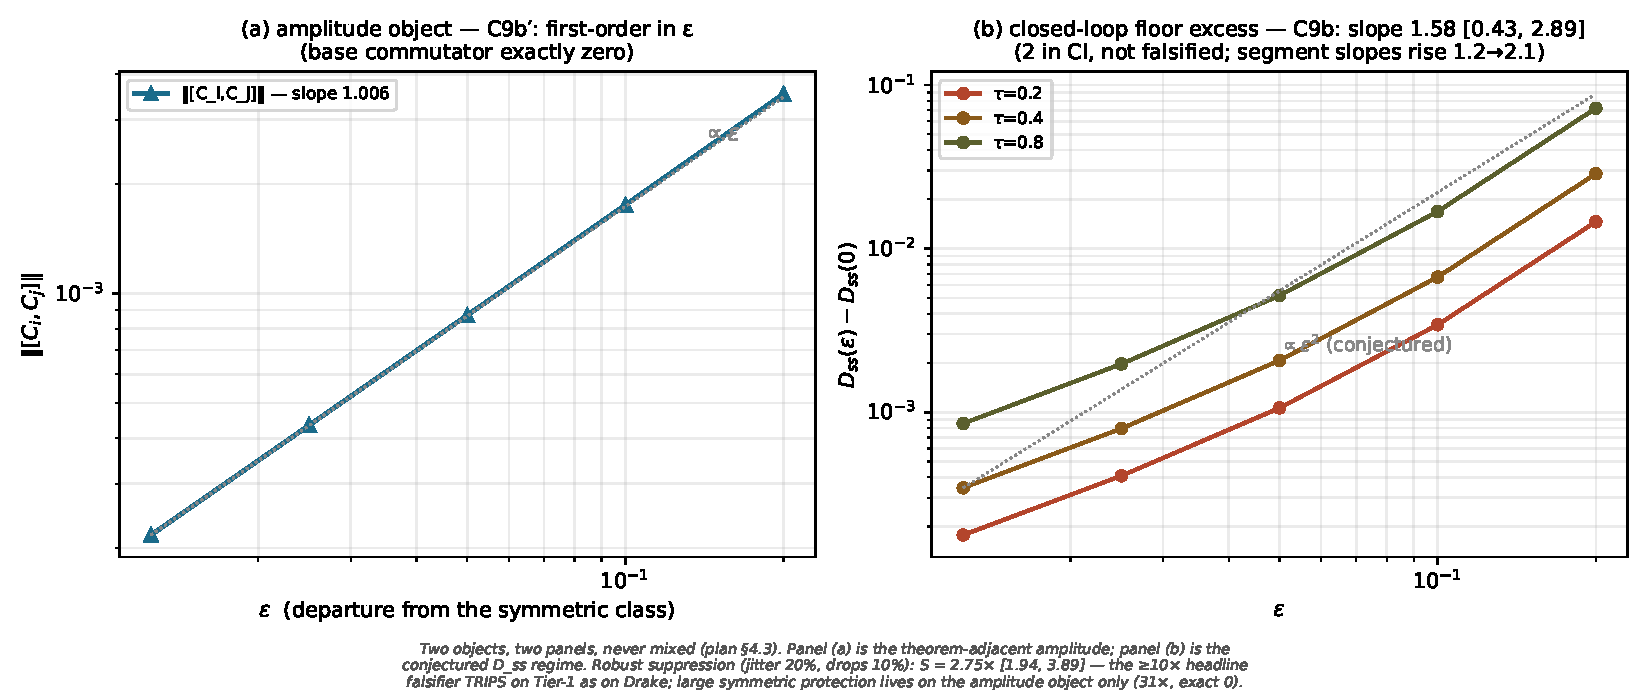
\includegraphics[width=\linewidth]{figures/f5_symmetry.pdf}
  \caption{F5: amplitude (a) and closed-loop floor (b) $\varepsilon$-response,
  never mixed in one panel.}
  \label{fig:f5tc}
\end{figure}

\subsection{Contraction in its own domain (E2; Thm.~\ref{thm:contractF})}
\begin{figure}[t]
  \centering
  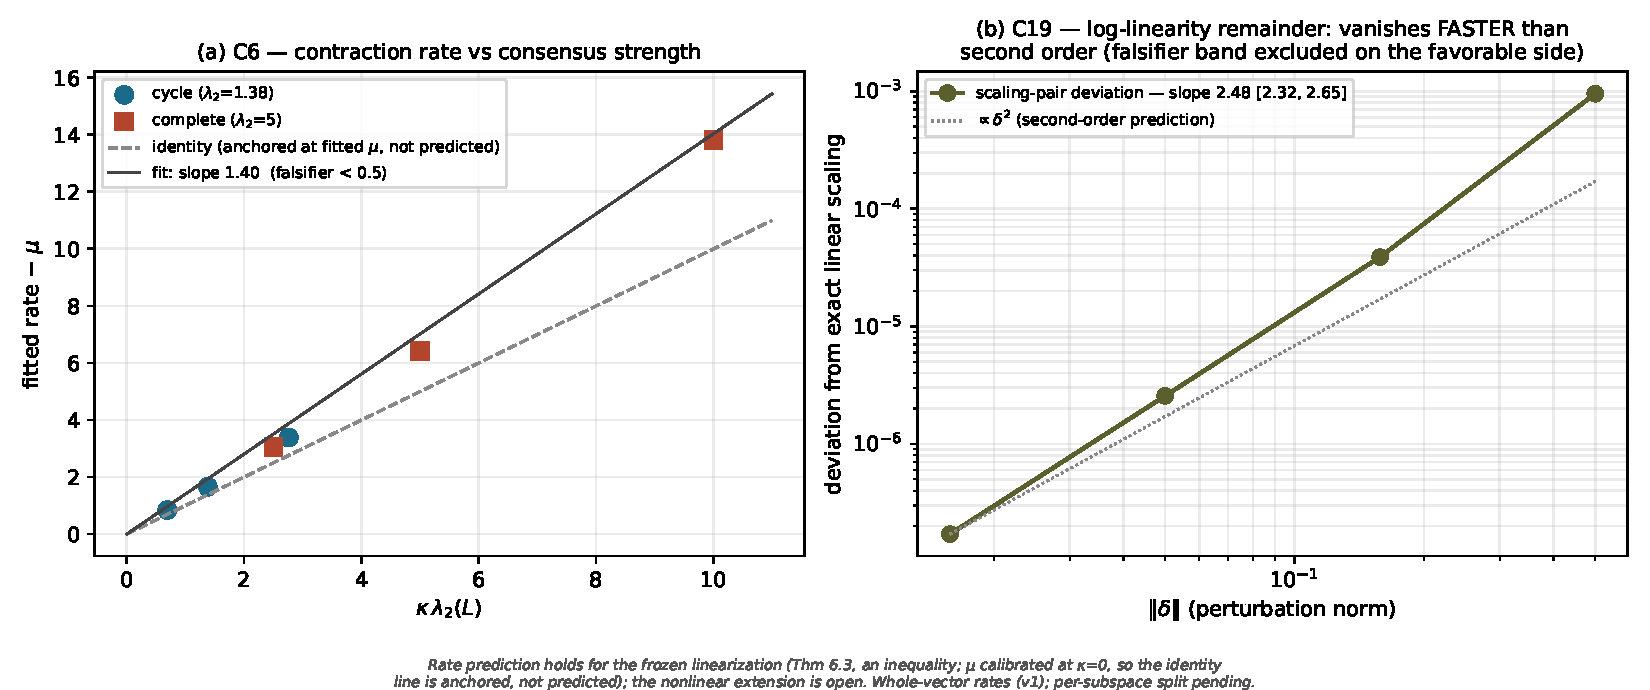
\includegraphics[width=\linewidth]{figures/f8_contraction.pdf}
  \caption{F8: rate versus $\kappa\lambda_2$ across two topologies, slope
  1.40 (falsifier $< 0.5$); $\mu$ calibrated at $\kappa = 0$, so the identity
  line is anchored, not predicted; the nonlinear extension is open.}
  \label{fig:f8tc}
\end{figure}
Step-perturbing all agents and fitting the decay of the gauge complement:
the rate scales with $\kappa\lambda_2$ at slope 1.403 across a $4\times$ gain
range and two topologies, with $\mu = -0.062$ topology-independent. The
log-linearity remainder vanishes \emph{faster} than the registered second
order (scaling-pair exponent 2.48 [2.32, 2.65]): the falsifier band is
excluded on the favorable side --- reported as tripped, with the corrected
order left to a restatement.

\subsection{Numerics invariance (E10)}
The excess exponent is invariant across integrator steps
$\Delta t \in \{0.001, 0.0025, 0.005, 0.01\}$\,s (all CIs share
$[1.185, 1.256]$), with the coefficient converging mildly under refinement:
no exponent above is an artifact of the discretization.

\subsection{Switch-off ladder}
\begin{table}[t]
\centering
\caption{Switch-off ladder (Tier-1 rows). Each arm kills the effect on
command or shifts its order as predicted.}
\begin{tabular}{lcc}
\toprule
arm & prediction & measured \\
\midrule
generic slope & $2$ & $1.999$ (formation-invariant $1.9993 \pm 0.0000$) \\
coefficient ratio ($m{=}2$) & $1$ & $1.0000$ \\
$s_i \equiv s_j$ & $0$ & $< 10^{-15}$ \\
level set $C_i = C_j$, sep $\ge 1$ & --- & full holonomy $\equiv 0$ (observed) \\
$\eta = 0$ & $0$ & $< 10^{-17}$ \\
$\xi = 0$ & $0$ & $0.0$ \\
$\tau = 0$ (explicit arm) & $0$ & $0.0$ \\
frozen shapes, closed loop & null & $D_{ss} \sim 10^{-30}$ \\
\bottomrule
\end{tabular}
\end{table}

\subsection{Reproducibility}
Every number in this section traces to a seeded, versioned driver and a
committed record; the released \texttt{campaign\_replay.py} re-executes
per-run probes that must match the records exactly (Tier-1 to $10^{-9}$). The
multibody campaign, its falsifications, and the cross-tier equivalence tests
appear in the RA-L companion.
